
%(BEGIN_QUESTION)
% Copyright 2009, Tony R. Kuphaldt, released under the Creative Commons Attribution License (v 1.0)
% This means you may do almost anything with this work of mine, so long as you give me proper credit

Examine this P\&ID and answer the following questions:

$$\includegraphics[width=15.5cm]{i04198x01.eps}$$

\vskip 10pt

Identify the ``normal'' mode of operation for this system: the status of the process valve and of the solenoid valve.

\vskip 10pt

Identify the ``normal'' mode of operation for the solenoid valve as specified by the solenoid manufacturer: the status of the solenoid valve when it is in a condition of rest (no stimulation).

\vskip 10pt

Explain what type of electrical signal status (power applied or power removed) is required at the solenoid valve to force a ``fail'' state at the process valve.

\vskip 20pt \vbox{\hrule \hbox{\strut \vrule{} {\bf Suggestions for Socratic discussion} \vrule} \hrule}

\begin{itemize}
\item{} The usage of the word ``normal'' is very different when describing a solenoid coil's energization state versus when the same word is used to describe a spring-return valve being ``normally-open'' or ``normally-closed.''  Explain how these two meanings differ, and why this distinction -- though confusing it may be -- is important to understand.
\item{} Identify the type of process valve used in this system, from the symbol.
\item{} If you have studied mathematical probability as it applies to system reliability, calculate the probability of the process valve shutting off when it shouldn't (i.e. this trip system's {\it unsecurity}) given the following probabilities of component failure:
\itemitem{} $P$ of solenoid valve passing air when commanded = 0.95
\itemitem{} $P$ of instrument air supply maintaining good pressure = 0.99
\itemitem{} $P$ of solenoid control signal remaining energized when it should = 0.985
\end{itemize}

\underbar{file i04198}
%(END_QUESTION)





%(BEGIN_ANSWER)


%(END_ANSWER)





%(BEGIN_NOTES)

The design engineer made it so that air will pass from the I/P to the process valve actuator during typical (good) operating conditions.  

\vskip 10pt

De-energization of the solenoid valve is what will cause the process valve to go to its fail state, which in this case is closed because the valve is labeled air-to-open (ATO).









\vskip 20pt \vbox{\hrule \hbox{\strut \vrule{} {\bf Virtual Trip-testing} \vrule} \hrule}

This question is a good candidate for a ``Virtual Trip-testing'' exercise.  Presenting the diagram to students, you pose an assignment whereby students must figure out how to test some component of this system to check that it will operate as intended to shut down the system in an abnormal (trip) condition, with some realistic limitation (e.g. power cannot be shut off to the load).  Students then propose various methods for executing the test.  Your job is to determine whether or not their proposed tests will achieve the desired result(s).

During and after the exercise, it is good to ask students follow-up questions such as:

\begin{itemize}
\item{} Where might our planned test strategy go wrong?  In other words, what thing(s) might happen to foil our test, either to invalidate the results or to not honor the stated limitation(s)?
\item{} Suppose the limitation were different.  How would this affect our ability to carry out the test?
\item{} Is the last test strategy best one we could execute?
\end{itemize}



%INDEX% Final Control Elements, valve: fail-safe solenoids

%(END_NOTES)


